\section{Case Studies}
\label{sec:casestudies}

Aliquam erat volutpat. Nunc eleifend leo vitae magna. In id erat non orci
commodo lobortis. Proin neque massa, cursus ut, gravida ut, lobortis eget,
lacus. Sed diam. Praesent fermentum tempor tellus. Nullam tempus. Mauris ac
felis vel velit tristique imperdiet. Donec at pede. Etiam vel neque nec dui
dignissim bibendum. Vivamus id enim. Phasellus neque orci, porta a, aliquet
quis, semper a, massa. Phasellus purus. Pellentesque tristique imperdiet tortor.
Nam euismod tellus id erat.

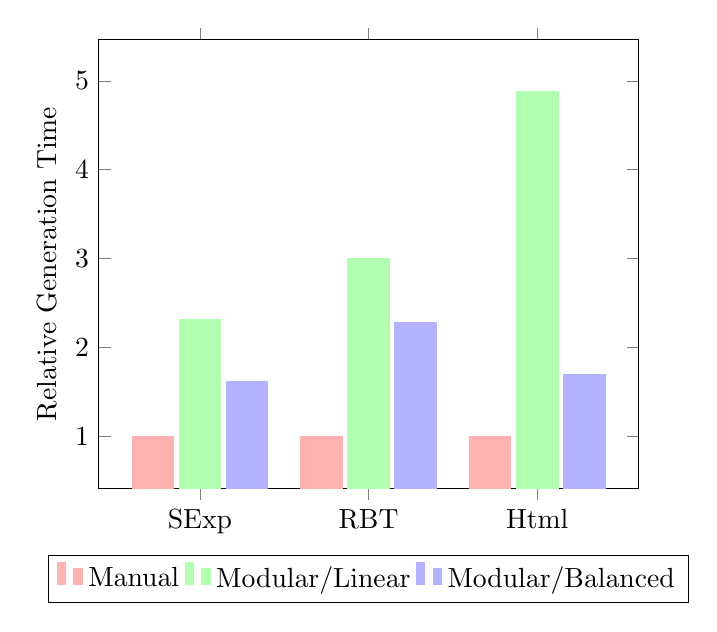
\begin{tikzpicture}
  \begin{axis}
    [ ybar
    , enlargelimits=0.15
    , enlarge x limits=0.3
    , /pgf/bar width=15pt
    , legend style={
        at={(0.5,-0.15)},
        anchor=north,legend columns=3}
    , ylabel={Relative Generation Time}
    , symbolic x coords={SExp, RBT, Html}
    , xtick=data
    % , nodes near coords
    , nodes near coords align={vertical}
    ]
    \addplot[fill, red!30]   coordinates {(SExp,1)    (RBT,1)    (Html,1)};
    \addplot[fill, green!30] coordinates {(SExp,2.31) (RBT,3)    (Html,4.88)};
    \addplot[fill, blue!30]  coordinates {(SExp,1.62) (RBT,2.28) (Html,1.70)};
    \legend{Manual, Modular/Linear, Modular/Balanced}
\end{axis}
\end{tikzpicture}